\documentclass{ximera}


\graphicspath{
  {./}
  {ximeraTutorial/}
  {basicPhilosophy/}
}

\newcommand{\mooculus}{\textsf{\textbf{MOOC}\textnormal{\textsf{ULUS}}}}


\usepackage{tkz-euclide}\usepackage{tikz}
\usepackage{tikz-cd}
\usetikzlibrary{arrows}
\tikzset{>=stealth,commutative diagrams/.cd,
  arrow style=tikz,diagrams={>=stealth}} %% cool arrow head
\tikzset{shorten <>/.style={ shorten >=#1, shorten <=#1 } } %% allows shorter vectors

\usetikzlibrary{backgrounds} %% for boxes around graphs
\usetikzlibrary{shapes,positioning}  %% Clouds and stars
\usetikzlibrary{matrix} %% for matrix
\usepgfplotslibrary{polar} %% for polar plots
\usepgfplotslibrary{fillbetween} %% to shade area between curves in TikZ
\usetkzobj{all}
\usepackage[makeroom]{cancel} %% for strike outs
%\usepackage{mathtools} %% for pretty underbrace % Breaks Ximera
%\usepackage{multicol}
\usepackage{pgffor} %% required for integral for loops



%% http://tex.stackexchange.com/questions/66490/drawing-a-tikz-arc-specifying-the-center
%% Draws beach ball
\tikzset{pics/carc/.style args={#1:#2:#3}{code={\draw[pic actions] (#1:#3) arc(#1:#2:#3);}}}



\usepackage{array}
\setlength{\extrarowheight}{+.1cm}
\newdimen\digitwidth
\settowidth\digitwidth{9}
\def\divrule#1#2{
\noalign{\moveright#1\digitwidth
\vbox{\hrule width#2\digitwidth}}}
























%%This is to help with formatting on future title pages.
\newenvironment{sectionOutcomes}{}{}


\title{Sine \& Cosine}

\begin{document}

\begin{abstract}
around the unit circle
\end{abstract}
\maketitle








For every angle, $\theta$, measured counterclockwise from the positive $x$-axis, we have a point on the unit circle. The coordinates of these points are functions of $\theta$.  We call them \textbf{cosine} and \textbf{sine}.






\begin{image}
\begin{tikzpicture}
  \begin{axis}[
            xmin=-1.1,xmax=1.1,ymin=-1.1,ymax=1.1,
            axis lines=center,
            width=4in,
            xtick={-1,1},
            ytick={-1,1},
            clip=false,
            unit vector ratio*=1 1 1,
            xlabel=$x$, ylabel=$y$,
            ticklabel style={font=\scriptsize},
            every axis y label/.style={at=(current axis.above origin),anchor=south},
            every axis x label/.style={at=(current axis.right of origin),anchor=west},
          ]        
          \addplot [smooth, domain=(0:360)] ({cos(x)},{sin(x)}); %% unit circle

          \addplot [textColor] plot coordinates {(0,0) (.766,.643)}; %% 40 degrees

          \addplot [ultra thick,penColor] plot coordinates {(.766,0) (.766,.643)}; %% 40 degrees
          \addplot [ultra thick,penColor2] plot coordinates {(0,0) (.766,0)}; %% 40 degrees
          
          %\addplot [ultra thick,penColor3] plot coordinates {(1,0) (1,.839)}; %% 40 degrees          

          \addplot [textColor,smooth, domain=(0:40)] ({.15*cos(x)},{.15*sin(x)});
          %\addplot [very thick,penColor] plot coordinates {(0,0) (.766,.643)}; %% sector
          %\addplot [very thick,penColor] plot coordinates {(0,0) (1,0)}; %% sector
          %\addplot [very thick, penColor, smooth, domain=(0:40)] ({cos(x)},{sin(x)}); %% sector
          \node at (axis cs:.15,.07) [anchor=west] {$\theta$};
          \node[penColor, rotate=-90] at (axis cs:.84,.322) {$\sin(\theta)$};
          \node[penColor2] at (axis cs:.383,0) [anchor=north] {$\cos(\theta)$};
          %\node[penColor3, rotate=-90] at (axis cs:1.06,.322) {$\tan(\theta)$};
        \end{axis}
\end{tikzpicture}
\end{image}




As the angle $\theta$ changes, sine and cosine oscillate between $-1$ and $1$.








\begin{image}
\begin{tikzpicture}
  \begin{axis}[
            domain=-10:10, ymax=1.5, xmax=10, ymin=-1.5, xmin=-10,
            axis lines =center, xlabel={$\theta$}, ylabel={$y$}, grid = major, grid style={dashed},
            ytick={-1.5,-1,-0.5,0.5,1,1.5},
            xtick={-7.85, -6.28, -4.71, -3.14, -1.57, 0, 1.57, 3.142, 4.71, 6.28, 7.85},
            xticklabels={$\tfrac{-5\pi}{2}$,$-2\pi$,$\tfrac{-3\pi}{2}$,$-\pi$, $\tfrac{-\pi}{2}$, $0$, $\tfrac{\pi}{2}$, $\pi$, $\tfrac{3\pi}{2}$, $2\pi$, $\tfrac{5\pi}{2}$},
            yticklabels={$1.5$,$-1$,$-0.5$,$0.5$,$1$,$1.5$}, 
            ticklabel style={font=\scriptsize},
            every axis y label/.style={at=(current axis.above origin),anchor=south},
            every axis x label/.style={at=(current axis.right of origin),anchor=west},
            axis on top
          ]
          

            \addplot [line width=2, penColor, smooth,samples=300,domain=(-10:10),<->] {sin(deg(x)};
            \addplot [line width=2, penColor2, smooth,samples=300,domain=(-10:10),<->] {cos(deg(x)};


            \node[penColor] at (axis cs:3.5,1.1) [anchor=north] {$\sin(\theta)$};
            \node[penColor2] at (axis cs:1.4,1.3) [anchor=north] {$\cos(\theta)$};



  \end{axis}
\end{tikzpicture}
\end{image}



Both are periodic functions with period $2\pi$.  Therefore, we can examine just one wave to understand the whole function.


Generally, people pick $[0, 2\pi)$ as the interval to investigate.





\begin{image}
\begin{tikzpicture}
  \begin{axis}[
            domain=0:7, ymax=1.5, xmax=7, ymin=-1.5, xmin=0,
            axis lines =center, xlabel={$\theta$}, ylabel={$y$}, grid = major, grid style={dashed},
            ytick={-1.5,-1,-0.5,0.5,1,1.5},
            xtick={1.57, 3.142, 4.71, 6.28, 7.85},
            xticklabels={$\tfrac{\pi}{2}$, $\pi$, $\tfrac{3\pi}{2}$, $2\pi$, $\tfrac{5\pi}{2}$},
            yticklabels={$1.5$,$-1$,$-0.5$,$0.5$,$1$,$1.5$}, 
            ticklabel style={font=\scriptsize},
            every axis y label/.style={at=(current axis.above origin),anchor=south},
            every axis x label/.style={at=(current axis.right of origin),anchor=west},
            axis on top
          ]
          

            \addplot [line width=2, penColor, smooth,samples=300,domain=(0:6.28)] {sin(deg(x)};
            \addplot [line width=2, penColor2, smooth,samples=300,domain=(0:6.28)] {cos(deg(x)};

            \addplot [color=penColor,only marks,mark=*] coordinates{(0,0)};
            \addplot [color=penColor,fill=white,only marks,mark=*] coordinates{(6.28,0)};
            \addplot [color=penColor2,only marks,mark=*] coordinates{(0,1)};
            \addplot [color=penColor2,fill=white,only marks,mark=*] coordinates{(6.28,1)};

            \node[penColor] at (axis cs:2.8,1.1) [anchor=north] {$\sin(\theta)$};
            \node[penColor2] at (axis cs:0.5,1.3) [anchor=north] {$\cos(\theta)$};

  \end{axis}
\end{tikzpicture}
\end{image}





We can see that sine and cosine have similar characteristics, just shifted.


\section*{Characteristics}





Picture the radius spinning counterclockwise around the unit circle.  The corresponding point on the unit circle will travel counterclockwise around the circle.  As the point moves around the circle, its coordinates oscillates between $-1$ and $1$.



The sine function collects the vertical coordinates.


\begin{center}
\desmos{m7devoo2w7}{400}{300}
\end{center}

As the point revolves counterclockwise around the unit circle, the values of sine 

\begin{itemize}
\item begin at $0$ at an angle of $0$
\item increase up to a maximum value of $1$ at an angle of $\frac{\pi}{2}$ (a quarter of the way around the circle)
\item decrease to $0$ at an angle of $\pi$ (halfway way around the circle)
\item continue decreasing to a minimum value of $-1$ at an angle of $\frac{3 \pi}{2}$ (three-quarters of the way around the circle)
\item increase back to $0$ at an angle of $2 \pi$ (a full circle around)
\end{itemize}










The cosine function collects the horizontal coordinates.

\begin{center}
\desmos{3t8cjtu1ak}{400}{300}
\end{center}

As the point revolves counterclockwise around the unit circle, the values of cosine 

\begin{itemize}
\item begin at a maximum value of $1$ at an angle of $0$
\item decrease to a value of $0$ at an angle of $\frac{\pi}{2}$ (a quater of the way around the circle)
\item continue decreasing to a minimum value of $-1$ at an angle of $\pi$ (halfway around the circle)
\item increasing to a value of $0$ at an angle of $\frac{3 \pi}{2}$ (three-quaters of the way around the circle)
\item continue increasing back to $1$ at an angle of $2 \pi$ (a full circle around)
\end{itemize}


















\subsection*{Easy Angles}





Sine and cosine are \textbf{transcendental functions}.  They transcend Algebra. They are beyond our algebraic tools.  That makes equations difficult when they involve sine and cosine.


This is true unless you work with angles that just happen to have nice values for sine and cosine.  We have several: $30^{\circ}$, $45^{\circ}$, and $60^{\circ}$.




\begin{itemize}
\item $\sin(30^{\circ}) = \frac{1}{2}$
\item $\cos(30^{\circ}) = \frac{\sqrt{3}}{2}$
\end{itemize}


And, since $30^{\circ}$ and $60^{\circ}$ make up a right triangle, we have 


\begin{itemize}
\item $\sin(60^{\circ}) = \frac{\sqrt{3}}{2}$
\item $\cos(60^{\circ}) = \frac{1}{2}$
\end{itemize}




$45^{\circ}$ cuts the quadrant in half making sine and cosine equal.

\begin{itemize}
\item $\sin(45^{\circ}) = \frac{1}{\sqrt{2}}$
\item $\cos(45^{\circ}) = \frac{1}{\sqrt{2}}$
\end{itemize}



Add these to $0^{\circ}$, $90^{\circ}$, $180^{\circ}$, and $270^{\circ}$ and we can walk around the unit circle.






  \begin{image}
    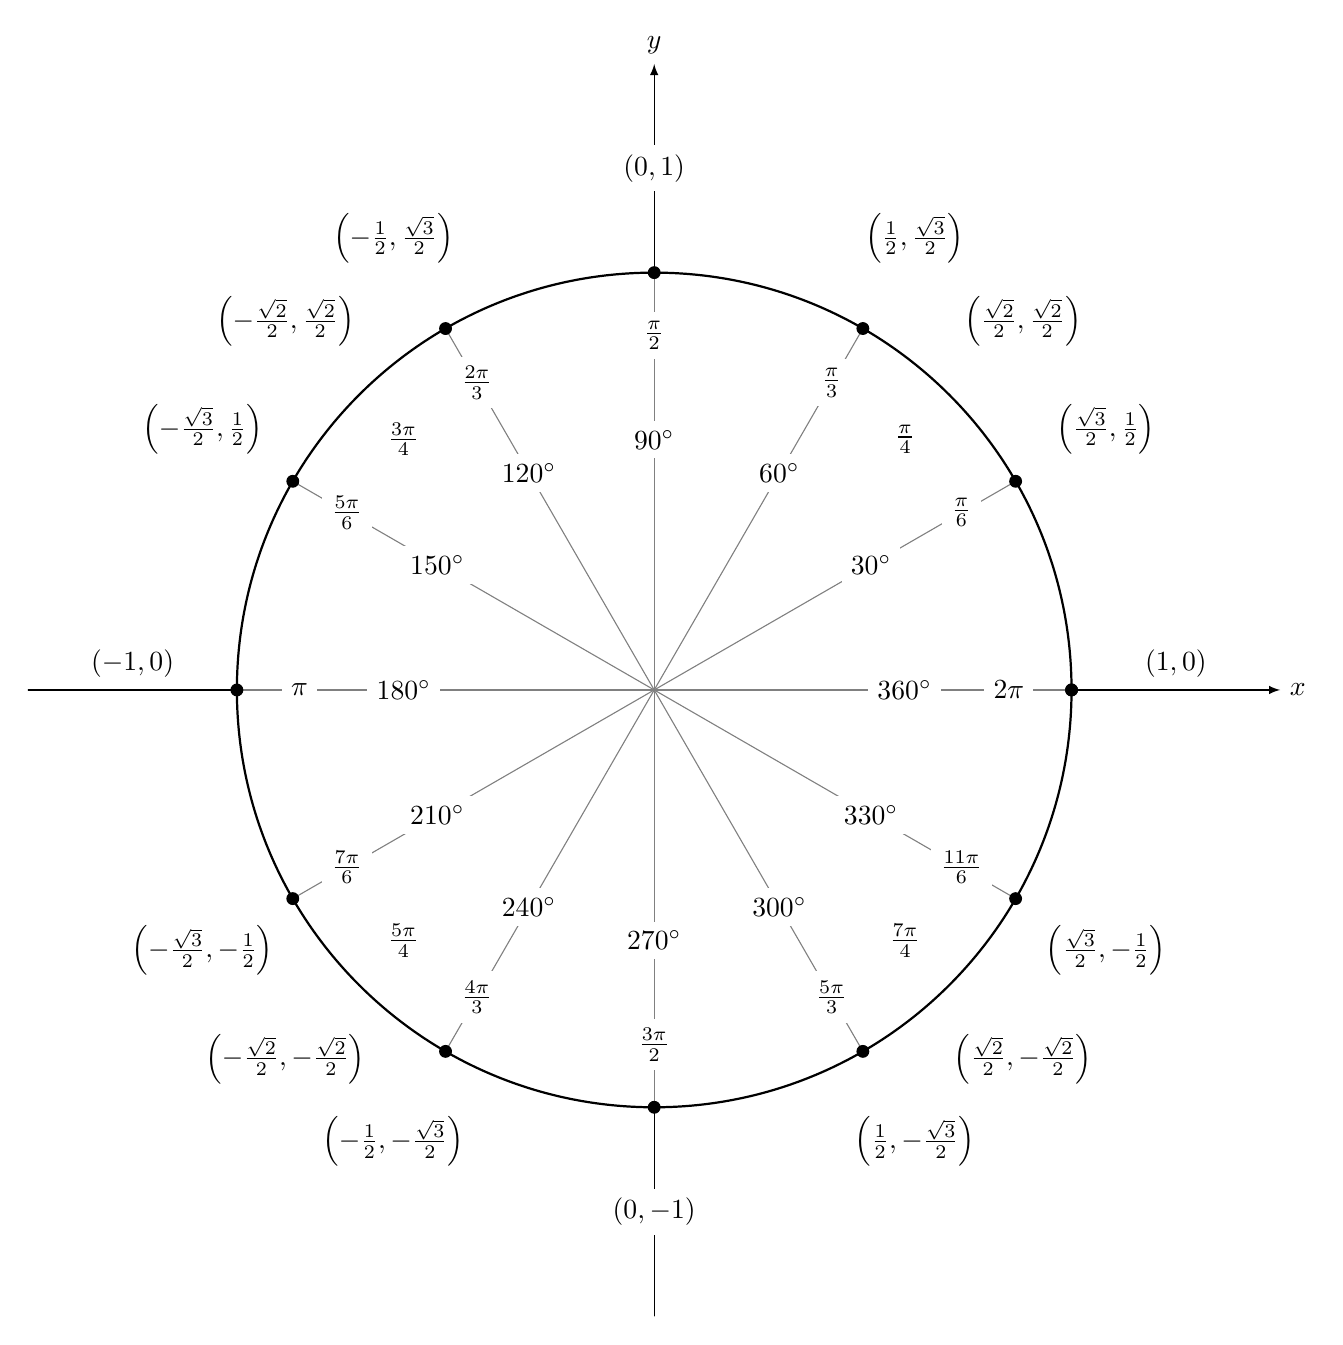
\begin{tikzpicture}[scale=5.3,cap=round,>=latex]
        % draw the coordinates
        \draw[->] (-1.5cm,0cm) -- (1.5cm,0cm) node[right,fill=white] {$x$};
        \draw[->] (0cm,-1.5cm) -- (0cm,1.5cm) node[above,fill=white] {$y$};

        % draw the unit circle
        \draw[thick] (0cm,0cm) circle(1cm);

        \foreach \x in {0,30,...,360} {
                % lines from center to point
                \draw[gray] (0cm,0cm) -- (\x:1cm);
                % dots at each point
                \filldraw[black] (\x:1cm) circle(0.4pt);
                % draw each angle in degrees
                \draw (\x:0.6cm) node[fill=white] {$\x^\circ$};
        }

        % draw each angle in radians
        \foreach \x/\xtext in {
            30/\frac{\pi}{6},
            45/\frac{\pi}{4},
            60/\frac{\pi}{3},
            90/\frac{\pi}{2},
            120/\frac{2\pi}{3},
            135/\frac{3\pi}{4},
            150/\frac{5\pi}{6},
            180/\pi,
            210/\frac{7\pi}{6},
            225/\frac{5\pi}{4},
            240/\frac{4\pi}{3},
            270/\frac{3\pi}{2},
            300/\frac{5\pi}{3},
            315/\frac{7\pi}{4},
            330/\frac{11\pi}{6},
            360/2\pi}
                \draw (\x:0.85cm) node[fill=white] {$\xtext$};

        \foreach \x/\xtext/\y in {
            % the coordinates for the first quadrant
            30/\frac{\sqrt{3}}{2}/\frac{1}{2},
            45/\frac{\sqrt{2}}{2}/\frac{\sqrt{2}}{2},
            60/\frac{1}{2}/\frac{\sqrt{3}}{2},
            % the coordinates for the second quadrant
            150/-\frac{\sqrt{3}}{2}/\frac{1}{2},
            135/-\frac{\sqrt{2}}{2}/\frac{\sqrt{2}}{2},
            120/-\frac{1}{2}/\frac{\sqrt{3}}{2},
            % the coordinates for the third quadrant
            210/-\frac{\sqrt{3}}{2}/-\frac{1}{2},
            225/-\frac{\sqrt{2}}{2}/-\frac{\sqrt{2}}{2},
            240/-\frac{1}{2}/-\frac{\sqrt{3}}{2},
            % the coordinates for the fourth quadrant
            330/\frac{\sqrt{3}}{2}/-\frac{1}{2},
            315/\frac{\sqrt{2}}{2}/-\frac{\sqrt{2}}{2},
            300/\frac{1}{2}/-\frac{\sqrt{3}}{2}}
                \draw (\x:1.25cm) node[fill=white] {$\left(\xtext,\y\right)$};

        % draw the horizontal and vertical coordinates
        % the placement is better this way
        \draw (-1.25cm,0cm) node[above=1pt] {$(-1,0)$}
              (1.25cm,0cm)  node[above=1pt] {$(1,0)$}
              (0cm,-1.25cm) node[fill=white] {$(0,-1)$}
              (0cm,1.25cm)  node[fill=white] {$(0,1)$};
    \end{tikzpicture}
  \end{image}




































\begin{center}
\textbf{\textcolor{green!50!black}{ooooo-=-=-=-ooOoo-=-=-=-ooooo}} \\

more examples can be found by following this link\\ \link[More Examples of Trigonometric Functions]{https://ximera.osu.edu/csccmathematics/precalculus/precalculus/trigFunctions/examples/exampleList}

\end{center}


\end{document}

